%%%%%%%%%%%%%%%%%%%%%%%%%%%%%%%%%%%%%%%%%%%%%%%%%%%%%%%%%%%%%%%%%%%%%%%%%%%%%%%%
%2345678901234567890123456789012345678901234567890123456789012345678901234567890
%        1         2         3         4         5         6         7         8

\documentclass[letterpaper, 10 pt, conference]{ieeeconf}  % Comment this line out
                                                          % if you need a4paper
%\documentclass[a4paper, 10pt, conference]{ieeeconf}      % Use this line for a4
                                                          % paper

\IEEEoverridecommandlockouts                              % This command is only
                                                          % needed if you want to
                                                          % use the \thanks command
\overrideIEEEmargins
% See the \addtolength command later in the file to balance the column lengths
% on the last page of the document

\usepackage{graphicx}
\usepackage{multicol}
\usepackage{subfigure}
\usepackage{mathptmx} % use Times fonts if available on your TeX system
\usepackage{setspace}

% The following packages can be found on http:\\www.ctan.org
%\usepackage{graphics} % for pdf, bitmapped graphics files
%\usepackage{epsfig} % for postscript graphics files
%\usepackage{mathptmx} % assumes new font selection scheme installed
%\usepackage{times} % assumes new font selection scheme installed
%\usepackage{amsmath} % assumes amsmath package installed
%\usepackage{amssymb}  % assumes amsmath package installed

\title{\LARGE \bf
Decentralized Communications for Self-regulated\\ Division of Labour in Robot Society
}

\author{ Md Omar Faruque Sarker and Torbjorn Dahl\\
         %\thanks{This research has been funded by the Engineering and Physical Sciences 				Research Council (EPSRC), UK, grant reference EP/E061915/1.}%
        Robotic Intelligence Lab, Newport Business School\\
		University of Wales, Newport, Allt-yr-yn Campus\\ 
		Allt-yr-yn Avenue, Newport, NP205XR, UK\\
		{\tt\small Mdomarfaruque.Sarker@newport.ac.uk}\\ 
		{\tt\small Torbjorn.Dahl@newport.ac.uk}      
}

%\author{Huibert Kwakernaak and Pradeep Misra% <-this % stops a space
%\thanks{This research has been funded by the Engineering and Physical Sciences Research Council (EPSRC), UK, grant reference EP/E061915/1.}% <-this % stops a space
%%\thanks{H. Kwakernaak is with Faculty of Electrical Engineering, Mathematics and Computer Science,
%%        University of Twente, 7500 AE Enschede, The Netherlands
%%        {\tt\small h.kwakernaak@autsubmit.com}}%
%%\thanks{P. Misra is with the Department of Electrical Engineering, Wright State University,
%%        Dayton, OH 45435, USA
%%        {\tt\small pmisra@cs.wright.edu}}%
%}


\begin{document}


\maketitle
\thispagestyle{empty}
\pagestyle{empty}


%%%%%%%%%%%%%%%%%%%%%%%%%%%%%%%%%%%%%%%%%%%%%%%%%%%%%%%%%%%%%%%%%%%%%%%%%%%%%%%%
\begin{abstract}

Distributed local communication is one of the essential means by which various social insects achieve their self-regulatory division of labour. Unlike centralized static communication, this communication mode enables individuals to respond to local changes more quickly and it generally produces steady-state convergence of self-regulated division of labour (DoL) in social insects. However, realizing this kind of communication in a distributed multi-robot system (DMRS) is not as straight forward as a centralized one. From a robot controller's point of view, it is not easy to determine how often or how much dynamic peer-to-peer (P2P) communication  is needed to maintain system's convergence of division of labour. In this paper, we address these questions: first by describing our model of local communication based DMRS with two different communication radii that shows a steady-state convergence of self-regulated DoL. Then we compare this system with our centralized communication based DMRS. All experiments on these systems  have been done with 16 physical E-puck robots in an area of about 2m x 2m. Results from these experiments suggest that faster and more stable convergence can be obtained by setting a smaller P2P communication radius where a robot locally exchanges signals with a minimum number of its closest peers.

\end{abstract}


%%%%%%%%%%%%%%%%%%%%%%%%%%%%%%%%%%%%%%%%%%%%%%%%%%%%%%%%%%%%%%%%%%%%%%%%%%%%%%%%
\section{INTRODUCTION}
\label{sec:intro}
%\vspace{2mm}
Multi-agent task allocation or division of labour (DoL) is a challenging research issue in the field of multi-agent and multi-robot systems e.g., swarm robotics \cite{RefSwarm}. In order to address this issue, existing approaches e.g., predefined (off-line) and emergent (real-time) task-allocation, fail to scale well with large number of agents. Typically, increased communication interference and decreased bandwidth among agents are major causes of this problem. Unlike the swarm robotic approach, which is inspired by biological systems alone and commonly aims for minimal intelligence agents, we propose to solve DoL in multi-agents based on a set of observed generic rules of DoL from biological and human social systems. These bottom-up rules describe the phenomena of self-regulated DoL in terms of attractive fields between agents and tasks. The concrete form of these rules, termed as \textit{attractive filed model} (AFM) \cite{RefElsa}, offers a scalable solution to the above DoL problem. Unlike having strong dependence to communication mediums by most of the existing approaches, our model states that self-regulatory DoL can be established by AFM without maintaining a strong form of on-line communication. 
%\vspace{4mm}
We have investigated the performance of two different communication strategies for self-regulated DoL among a larger robot teams: centralized and local. These forms of communications typically resemble to message broadcast and peer-to-peer (P2P) communications respectively.


%%%%%%%%%%%%%%%%%%%%%%%%%%%%%%%%%%%%%%%%%%%%%%%%%%%%%%%%%%%%%%%%%%%%%%%%%%%%%%%%
\section{Modeling}
\label{sec:model}
\subsection{Model for Self-Regulatory DoL}
Our model of self-regulated DoL is based on AFM. It provides us a generic framework for implementing self-regulatory DoL in robots. Here we briefly describe how this model gives our robots self-regulatory DoL behaviours, particularly task-specialization, concurrency, flexibility and robustness.
Let us consider a manufacturing shop floor scenario where N number of mobile robots are required to attend to M number of shop tasks spread over a fixed area A. Let these tasks be represented by a set of small rectangular boxes resembling to manufacturing machines. Let $R_1$, $R_2$ … $R_n$ be the set of all robots and $J_1$, $J_2$ … $J_m$ be the set of all tasks. Each task $j$ has an associated task-urgency $\phi_j$ that indicates its relative importance over time. If a robot attends to a task $j$ in x$^{th}$ time-step, value of $\phi_j$ will decreases by a small amount $\delta_\phi$ in (x+1)$^{th}$ time-step. On the other hand, if a task has not been served by any robot in x$^{th}$ time-step,  $\phi_j$  will increase by another small amount in (x+1)$^{th}$ time-step. In order to complete a shop task $J_1$, a robot $R_1$ needs to reach within a fixed boundary $D_j1$ of $J_1$. If a robot completes a task $j$ we say that it learns about it and this will increase robot's likelihood of selecting that task in next step. We call this variable affinity of a robot to that task as its sensitization $k_j$ . If a robot does not do a task $j$ for some time, we say that it forgets about $j$ and $k_j$ has been decreased.\\
According AFM, all robots will establish attractive fields to all tasks due to the presence of a system-wide continuous flow of information. The strength of these attractive fields called stimulus will vary according to the distances between robots and tasks, task-urgencies and corresponding  sensitizations of robots. This is encoded in Eq. \ref{eqn1}.
%\addtolength{\abovedisplayskip}{-15mm} 
\begin{small}
%\begin{multicols}{2} 
\begin{equation}
S_{j}^{i} = tanh\{\frac{k_{j}^{i}}{d+\delta } \phi _{j}\}
\label{eqn1}
\end{equation}
%\vspace*{0.25cm}
\begin{equation}
P_{j}^{i} = \frac{S_{j}^{i}}{\sum_{j}^{}S_{j}^{i}}
\label{eqn2}
\end{equation}
%\end{multicols}
\end{small}
%\addtolength{\belowdisplayskip}{-1mm} 
%\vspace{2mm}
Eqn \ref{eqn1} says that the stimuli of a robot $i$ to a particular task $j$, $(S_{j}^{i})$ depends on robot's spatial distance $d$ to $j$, level of sensitization to that task ($k_{j}^{i}$) and perceived urgency of that task ($\phi _{j}$). We use a vary small value $\delta$ in \ref{eqn1} to prevent  division by zero. The probability of selecting each task has been determined by a probabilistic method outlined in Eq. \ref{eqn2} . 
AFM suggests concurrency of a self-regulatory system by specifying at least two task options: 1) doing a task and 2) doing no task. In robots, the latter can be   be treated as random walking. So in any time-step a robot will choose from M+1 tasks. Let $T_a$ be the allocated time to accomplish a task. If $R_1$ can enter inside the task boundary within $T_a$ time it waits there until $T_a$ elapsed. Otherwise it will select a different task. 

\subsection{Model for Communication}
In order to establish a system-wide continuous flow of information, one needs to implement a  suitable communication system. Here we have presented two models of communication for our above manufacturing shop-floor scenario.
%
%\addtolength{\floatsep}{-25mm}
\begin{figure}[thpb]
\centering
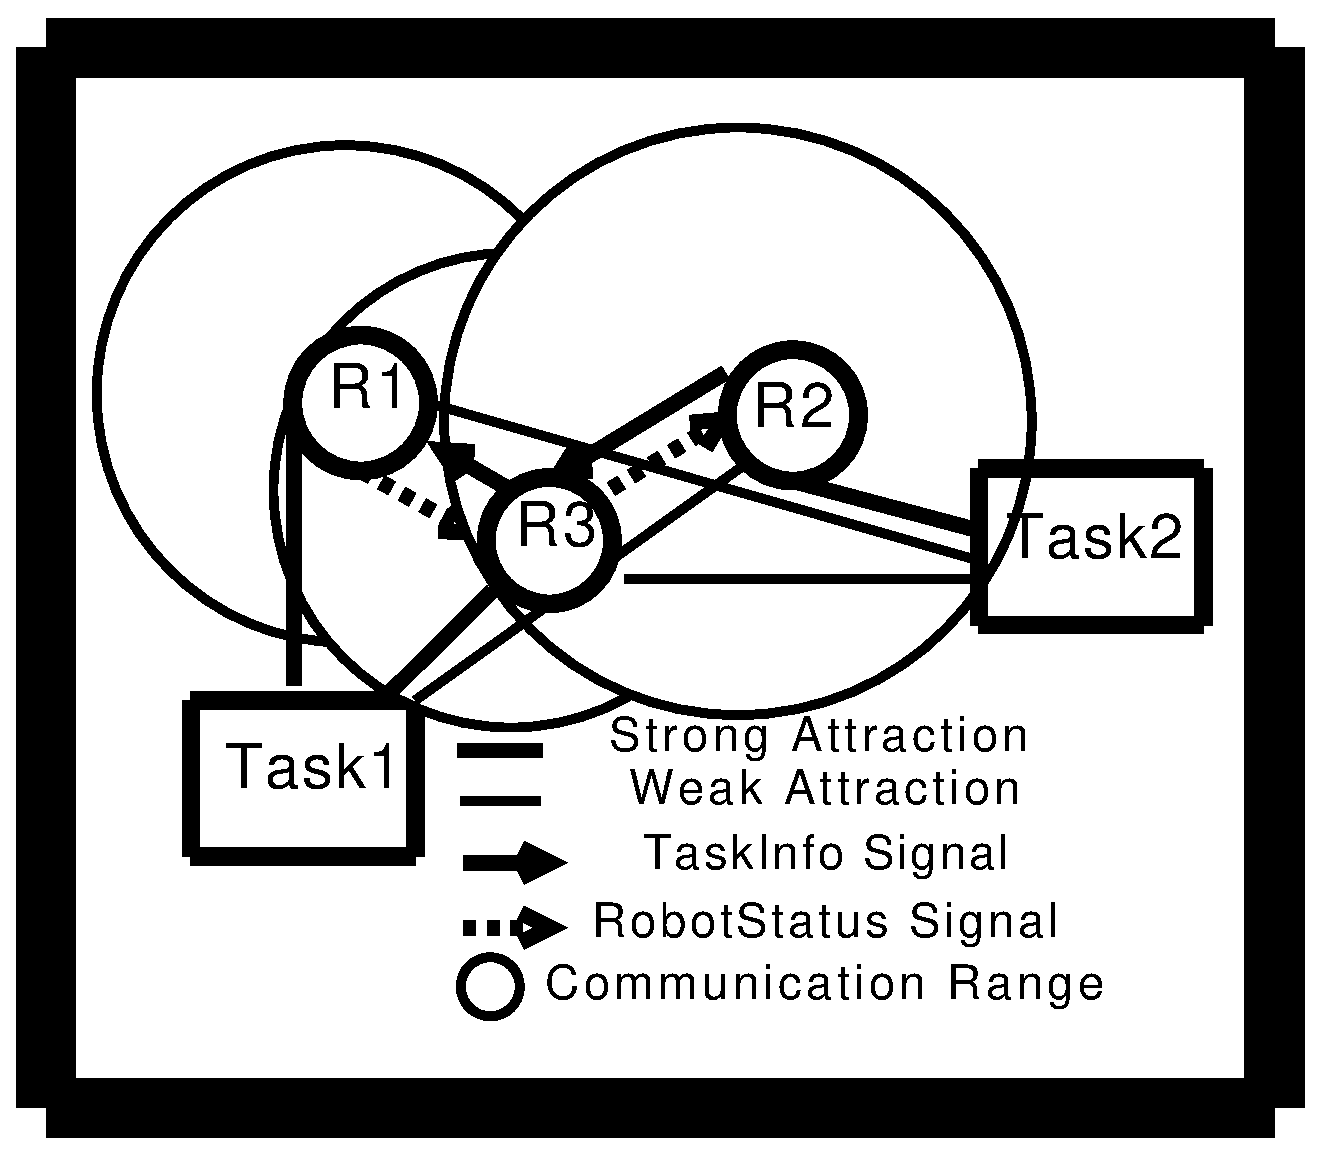
\includegraphics[height=4cm, angle=0]{../dia-files/LocalComm.eps}
% figure caption is below the figure
%\vspace*{0.20cm}
\caption{Local communication model}
\label{fig:lcm} % Give a unique label
\end{figure}
%\addtolength{\belowcaptionskip}{-15mm}
%\end{spacing}
%
\paragraph{Local Communication Model:}
This model is based on the P2P communications among robots. Here there is no centralized server to disseminate information but each robot can communicate to its nearby peers within its communication radius, $R_{comm}$. Here by $R_{comm}$, we assume that within this distance robots can exchange communication signals reliably without any significant loss of information or delay. A robot $R_1$ is a nearby peer  of robot $R_2$, if spatial distance between $R_1$ and $R_2$ is less than its $R_{comm}$. 
As shown in Fig. \ref{fig:lcm}, local communication can also give robots similar task information as in centralized communication mode. It shows that  it is not necessary for each robot to communicate with every other robot to get information on all tasks. Since robots can random walk  and explore the environment we assume that for a reasonably high robot to space density, all task will be known to all robots after an initial exploration period. 
In order to update the urgency of a task, robots can estimate the number of robots working on a task either by using their sensory perception (e.g., camera)  or by doing local P2P communication. In Fig. ref{fig:lcm} we have shown that robots exchange both TaskInfo and RobotStatus signals to peers.
%%%%%%%%%%%%%%%%%%%%%%%%%%%%%%%%%%%%%%%%%%%%%%%%%%%%%%%%%%%%%%%%%%%%%%%%%%%%%%%%
\section{Implementation}
\label{sec:impl}
\begin{figure}
\centering
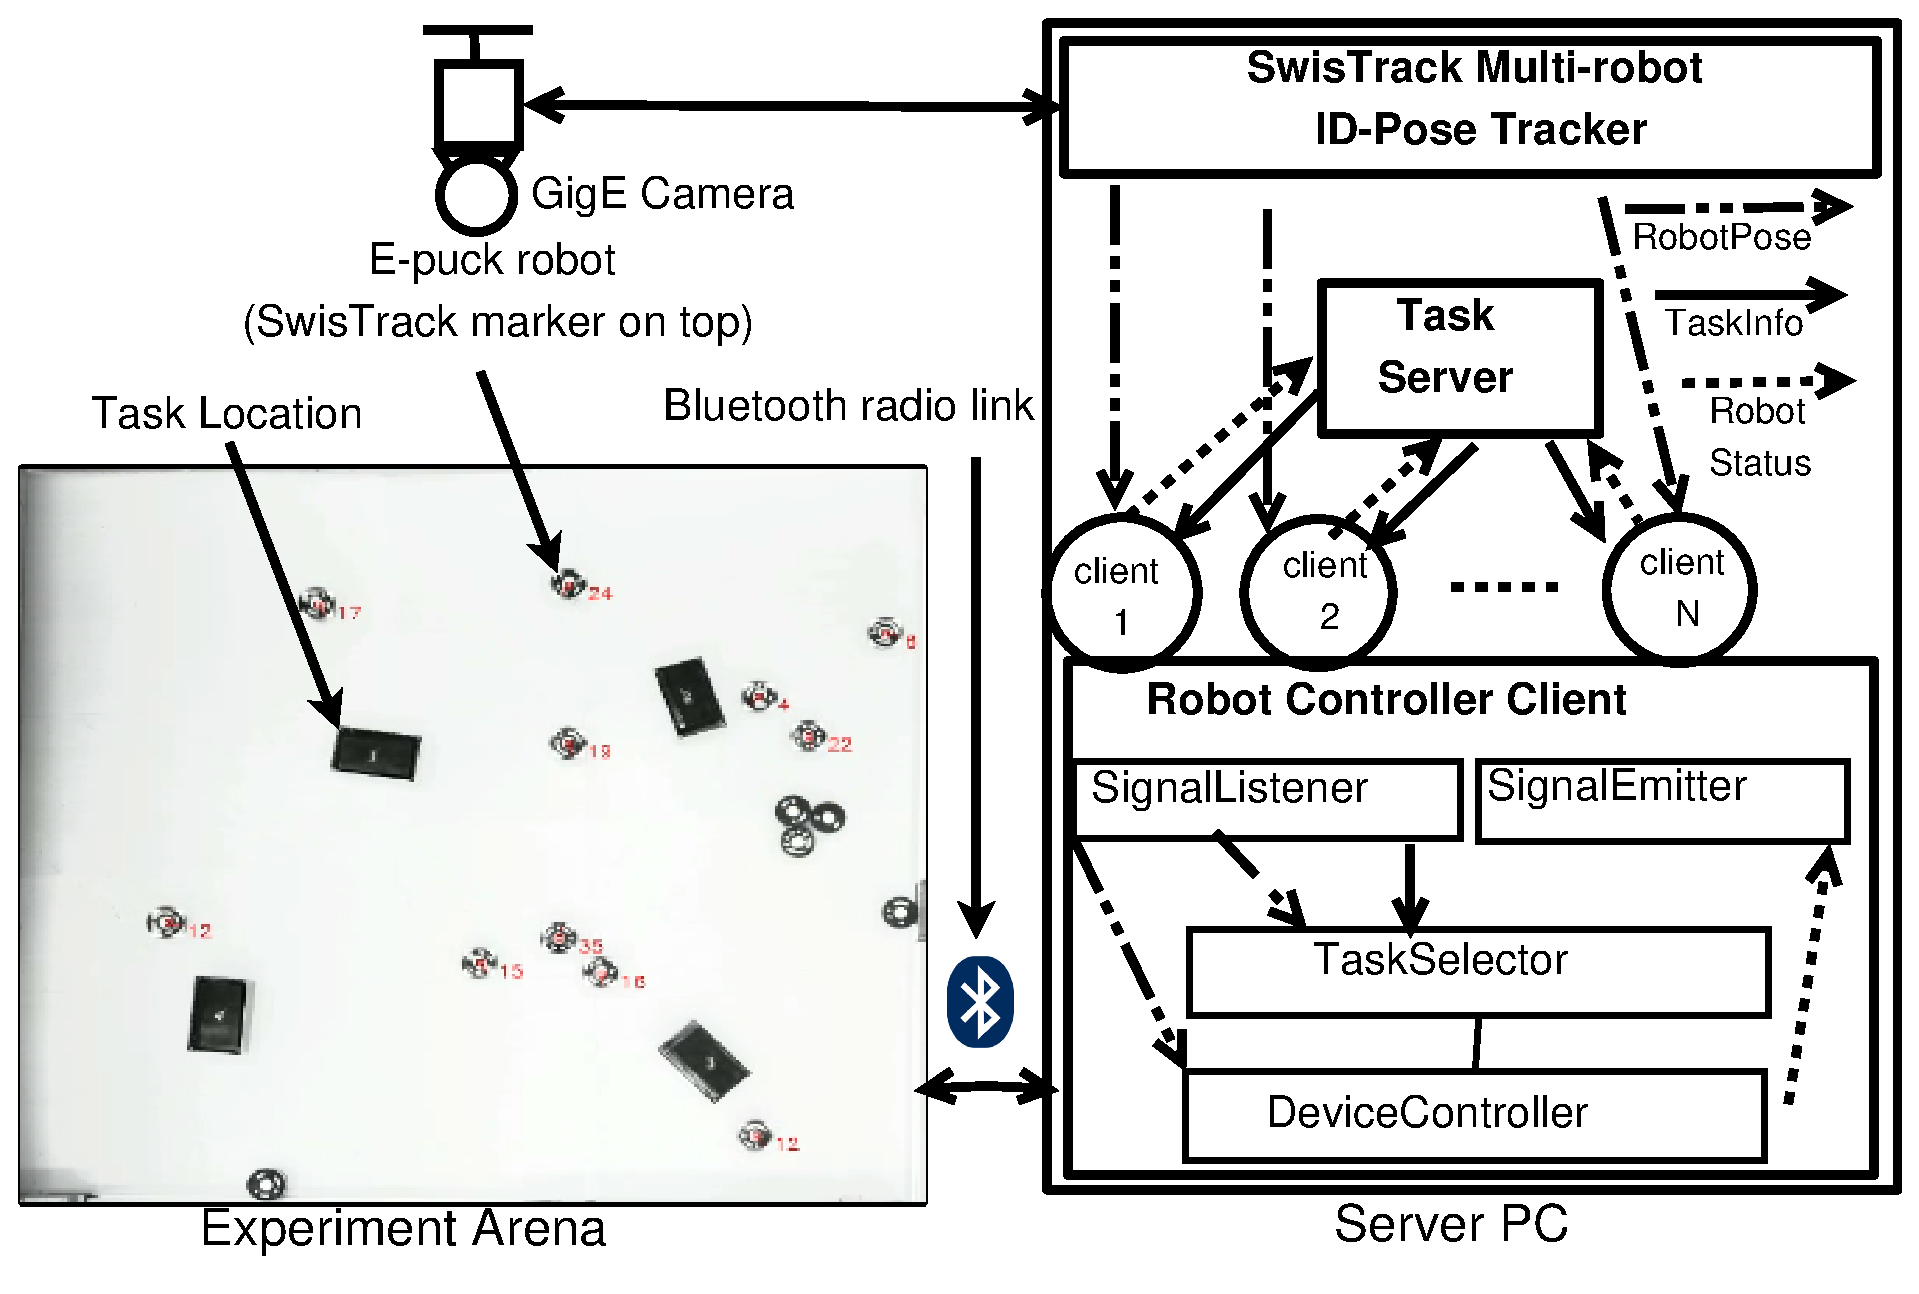
\includegraphics[height=5.5cm, angle=0]
{../dia-files/RIL-Expt-Setup1.eps}
%figure caption is below the figure
\caption{\small Hardware and software setup}
\label{fig:setup} % Give a unique label
\end{figure}
We have developed a system where up to 40 E-puck robots \cite{Epuck} can operate together according to the generic rules of the AFM. As shown in Fig. \ref{fig:setup}, our software system consists of a multi-robot tracking system, a centralized task server and robot controller clients. Here at first we have presented the design of our communication system. Then we have discussed about our specific implementation. 

%%%%%%%%%%%%%%%%%%%%%%%%%%%%%%%%%%%%%%%%%%%%%%%%%%%%%%%%%%%%%%%%%%%%%%%%%%%%%%%%%
\section{Experiment Design}
\label{sec:expt-design}
In this section, we have described the design of parameters and observables of our experiments.
These experiments are designed to validate AFM by testing the occurrence of convergent MRTA. Our experimental setup can be found in section~\ref{sec:impl}. The details of convergence is presented in section~\ref{sec:results}.
%
\begin{table}
\caption{Experimental parameters}
\label{table:params}
\begin{center}
\begin{tabular}{|l||c|}
\hline Parameter & Value\\
\hline Total number of robots ($N$) & 16\\
\hline Total number of tasks ($M$) & 4\\
\hline Experiment area ($A$) & 4 $m^2$\\
\hline Intial task urgency ($\Phi_{INIT}$) & 0.5\\
\hline Task urgency increase rate ($\Delta\phi_{INC}$) & 0.005\\
\hline Task urgency decrease rate ($\Delta\phi_{DEC}$) & 0.0025\\
\hline Intial sensitization ($K_{INIT}$) & 0.1\\
\hline Sensitization increase rate ($\Delta k_{INC}$) & 0.03\\
\hline Sensitization decrease rate ($\Delta k_{DEC}$) & 0.01\\
\hline A very small distance ($\delta$)& 0.000001\\
\hline Task info update interval ($\Delta TS_{u}$) & 5s\\
\hline Task info signal emission interval ($ \Delta TS_{e}$)& 2.5s\\
\hline Robot's task time-out interval ($\Delta RT_{to} $)& 10s\\
\hline
\end{tabular}
\end{center}
\end{table}
%%%%%%%%%%%%%%%%%%%%%%%%%%%%%%%%%%%%%%%%%%%%%%%%%%%%%%%%%%%%%%%%%%%%%%
\section{Results and Discussions}
\label{sec:results}
%%
In this section we have presented our experimental results. We ran those experiments for about 40 minutes and averaged them from three iterations.
%%% raw urgencies
\begin{figure}
\centering
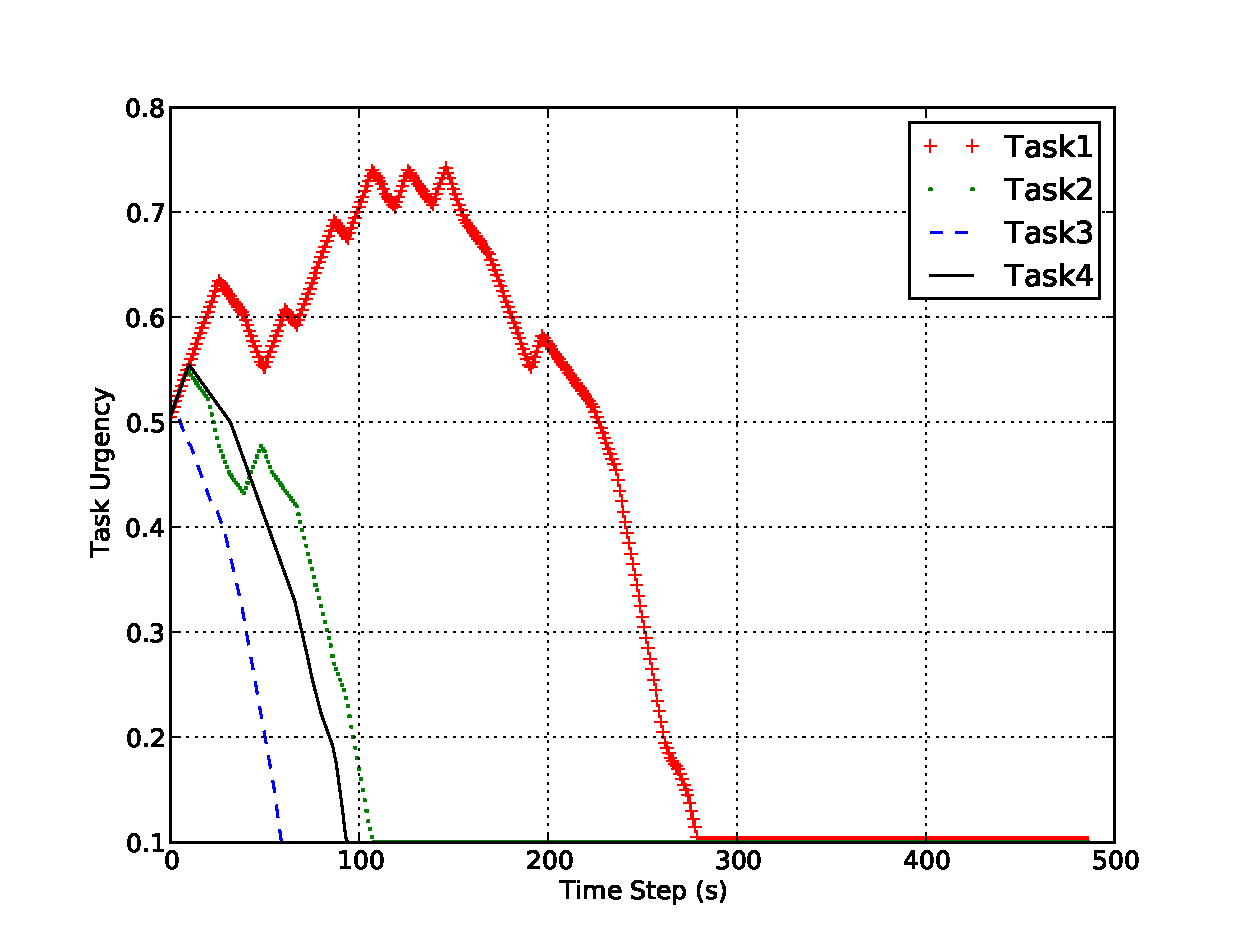
\includegraphics[height=5cm, angle=0]
{images/local-500cm/PlotUrgencyLog-2010Feb15-171017.eps}
%figure caption is below the figure
\caption{\small Task urgencies observed at TaskServer in local mode $R_{comm}$=0.5m}
\label{fig:raw-urgencies} % Give a unique label
\end{figure}
%%%
Fig. \ref{fig:raw-urgencies} shows the dynamic changes in task urgencies.
In order to describe our system's dynamic behaviour holistically we analyse the changes in task urgencies over time. Let $ \phi_{j, q}$ be the urgency of a task $j$ at $q^{th}$ step. In $(q+1)^{th}$ step, we can find the change of urgency of task $j$ :\\
\begin{equation} 
\small
\delta \phi_{j, q+1} = ( \phi_{j, q+1} - \phi_{j, q}) 
\end{equation}
So we can calculate the sum of changes in urgencies of all tasks at $(q+1)^{th}$ step:
\begin{equation} 
\small
\Delta \Phi_{j, q+1} = \sum_{j=1}^{M} \delta \phi_{j, q+1} 
\label{eqn:Delta-Phi}
\end{equation}
Fig. \ref{fig:urgency-convergence} plots this sum of changes of task urgencies by a dashed line. If we consider the absolute change over a window $w$ of time in the following equation we can describe the overall changes of our systems in both positive and negative directions.
%
\begin{equation}
\small
\Delta \Phi_{jw, q+1} = \sum_{j=0}^{w-1} \left | \Delta \Phi_{q+j} \right |
\end{equation}
%
In order to find convergence in DoL we have calculated the sum of absolute changes in task urgencies over a window of 2 consecutive steps (100s). This is plotted in solid line in Fig. \ref{fig:urgency-convergence}. Note that we scale down the time steps of this plot by aggregating the values of 10 consecutive steps (50s) of Fig. \ref{fig:raw-urgencies} into a single step value.
From Fig. \ref{fig:raw-urgencies} we can see that initially the sum of changes of task urgencies are towards negative direction. This implies that tasks are being served by a high number of robots. When the task urgencies stabilize near zero the fluctuations in urgencies become minimum. Since robots chose tasks stochastically, there will always be a small changes in task urgencies. A potential convergence point is shown in Fig. \ref{fig:urgency-convergence} by considering the persistence existence of the value of $\Delta \Phi_{jw, q+1}$ below a threshold 0.1. This convergence happens near step 23 or after 1150s from the beginning of our experiments. This implies that from this point of time and onwards, changes of our system's behaviour remains under a small threshold value.\\
%
Similar to Eq. \ref{eqn:Delta-Phi}, we can calculate the absolute sum of changes in sensitizations by all robots in the following equation.
% 
\begin{equation}
\small 
\Delta K_{j, q+1} = \sum_{j=1}^{M} \left | \Delta k_{j, q+1} \right |
\label{eqn:Delta-K}
\end{equation}
This values of $\Delta K$ are plotted in Fig. \ref{fig:sensitization-stat}. It shows that the overall rate of learning and forgetting decrease over time. It is a consequence of the gradually increased task specialization of robots.
%%%%
%%%%% Task Urgency Convergence
\begin{figure*}
\begin{minipage}[t]{0.5\linewidth}
\centering
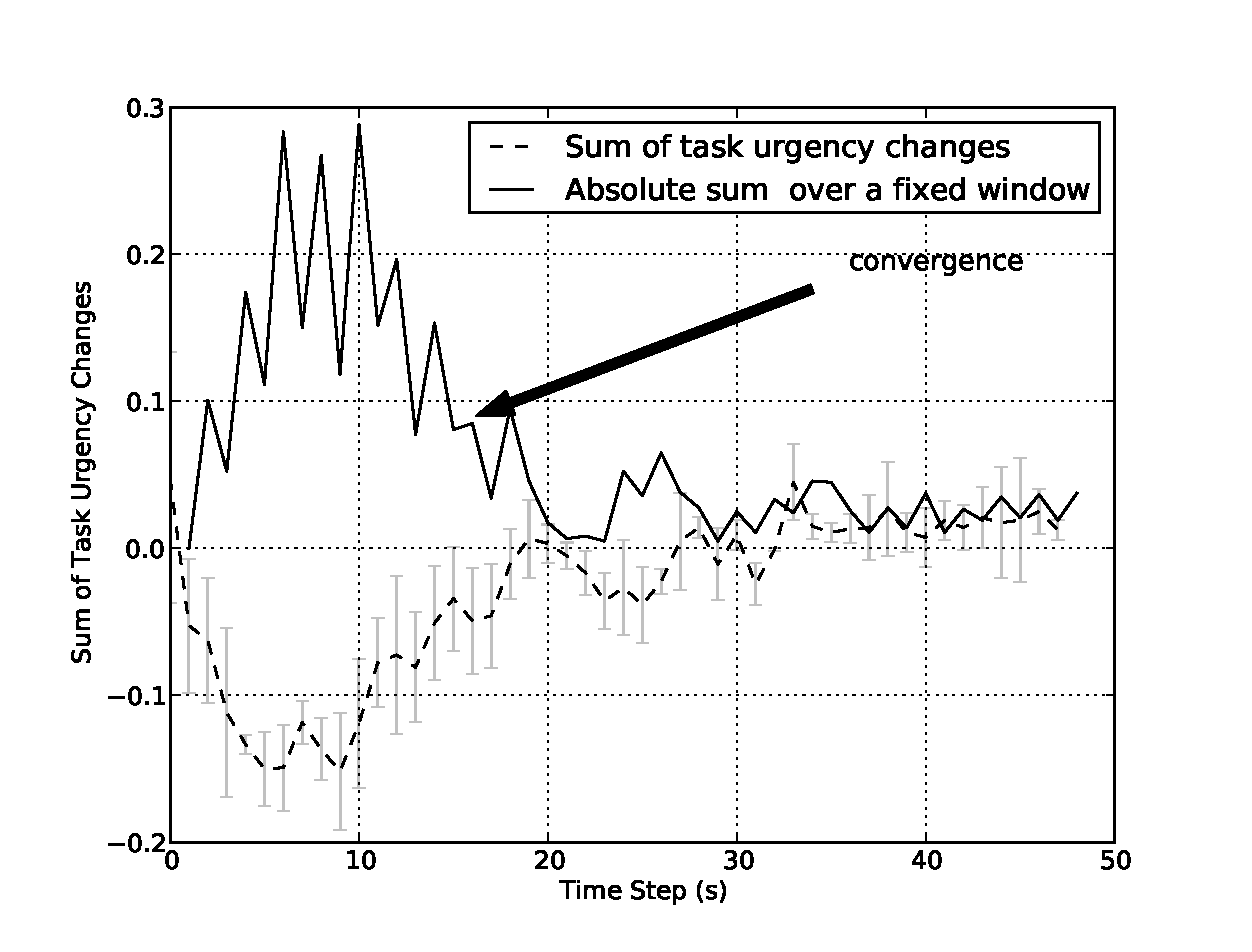
\includegraphics[height=5cm, angle=0]
{images/local-500cm/Local500cm-TaskUrgencyConvergence.eps}
%figure caption is below the figure
\caption{\small Convergence of task urgencies in local mode $R_{comm}$=0.5m}
\label{fig:l500cm-convergence} % Give a unique label
\end{minipage}
\hspace{0.5cm}
\begin{minipage}[t]{0.5\linewidth}
\centering
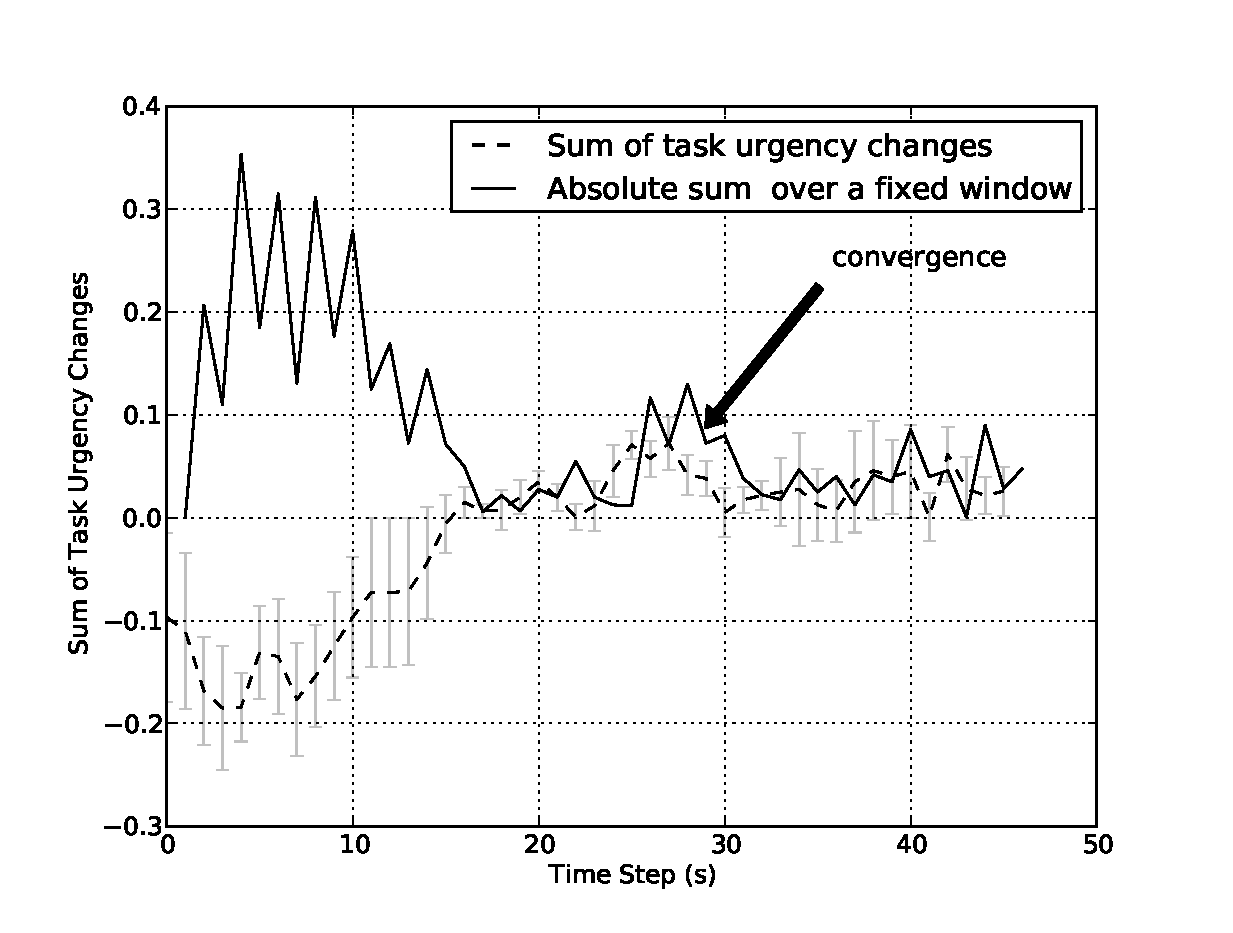
\includegraphics[height=5cm, angle=0]{images/local-1m/TaskUrgencyConvergence.eps}
\caption{\small Convergence of task urgencies in local mode $R_{comm}$=1m}
\label{fig:l1m-convergence} % Give a unique label
\end{minipage}
\end{figure*}
%%
%%% Sensitization%%%
\begin{figure*}
\begin{minipage}[t]{0.5\linewidth}
\centering
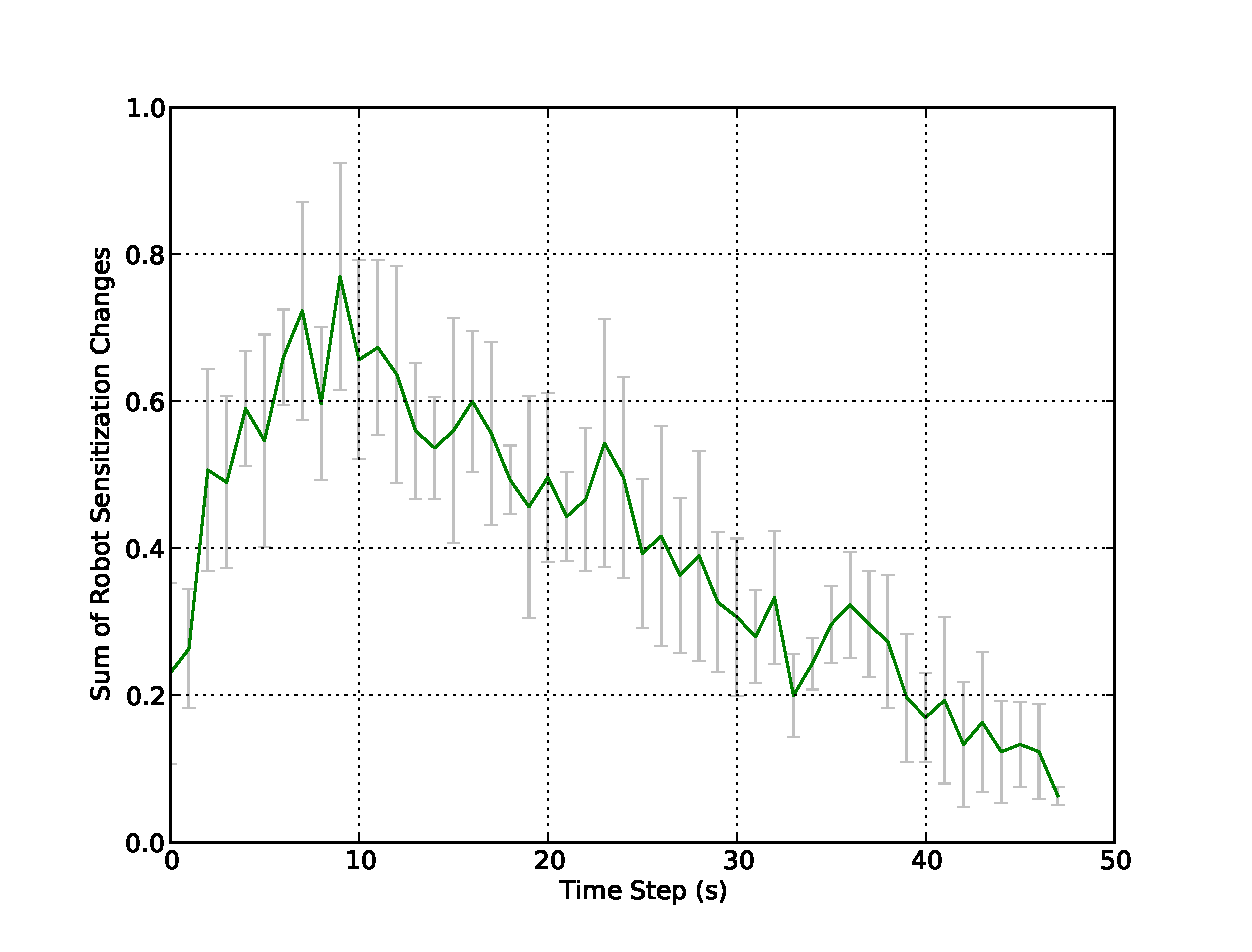
\includegraphics[height=5cm, angle=0]
{images/local-500cm/RobotSensitizationStat-Total-50steps.eps}
%figure caption is below the figure
\caption{\small Changes in sensitizations of all robots in local mode $R_{comm}$=0.5m}
\label{fig:sensitization-stat} % Give a unique label
\end{minipage}
\hspace{0.5cm}
\begin{minipage}[t]{0.5\linewidth}
\centering
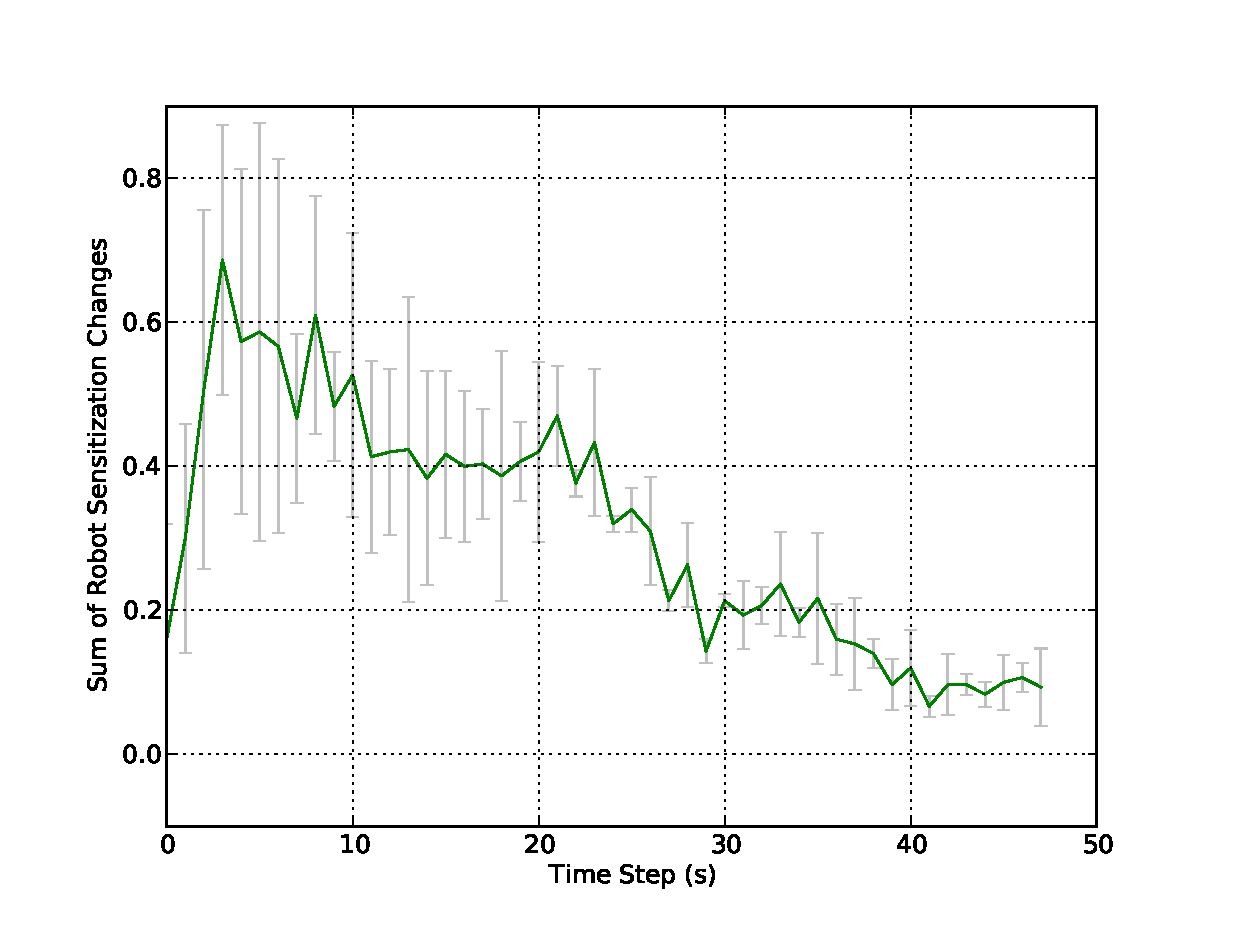
\includegraphics[height=5cm, angle=0]{images/local-1m/RobotSensitizationStat-Total-50steps.eps}
\caption{\small Changes in sensitizations of all robots in local mode $R_{comm}$=1m}
\label{fig:translation-stat} % Give a unique label
\end{minipage}
\end{figure*}
%%
%%% Translation %%%
\begin{figure*}
\begin{minipage}[t]{0.5\linewidth}
\centering
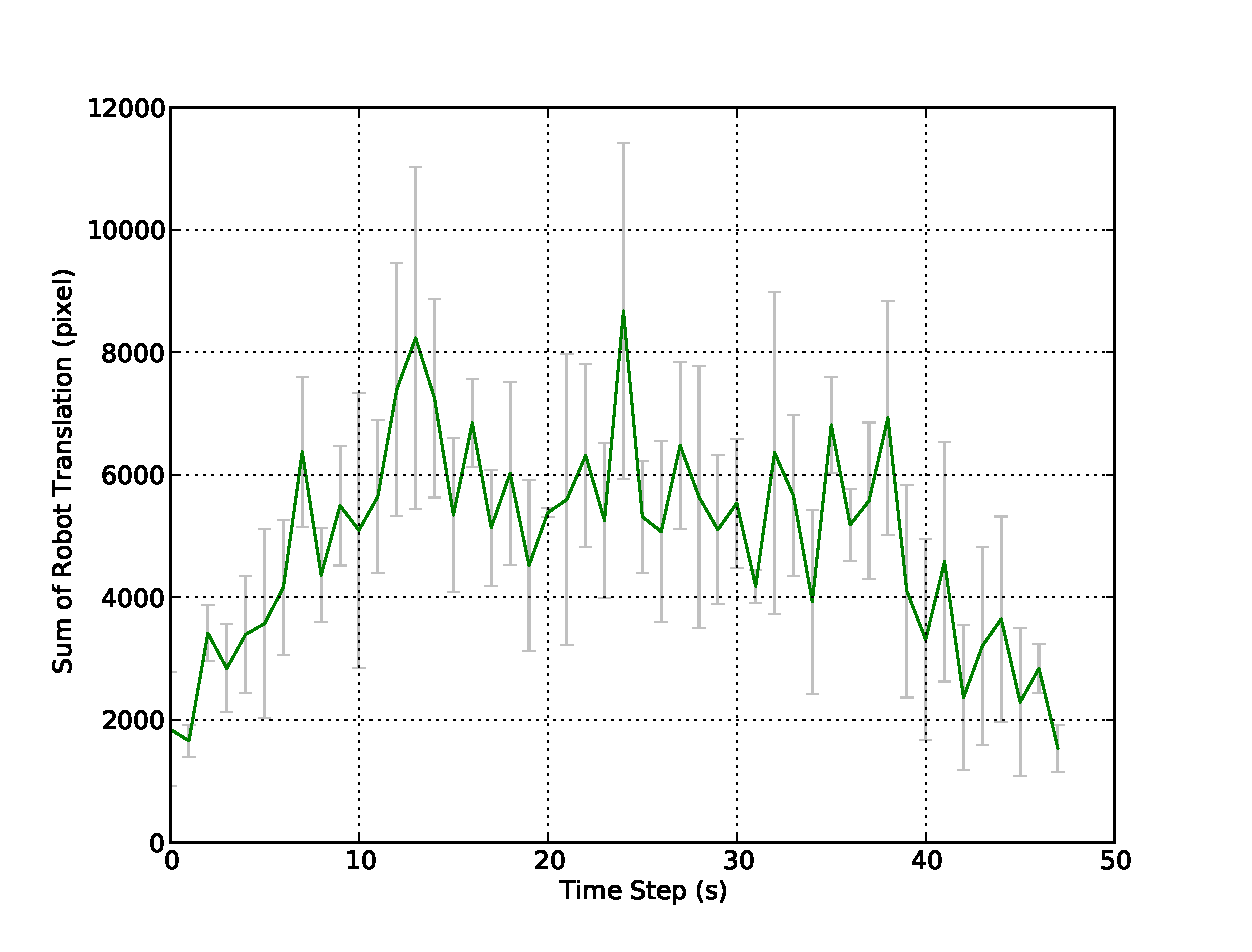
\includegraphics[height=5cm, angle=0]
{images/local-500cm/DeltaTranslationStat.eps}
%figure caption is below the figure
\caption{\small Sum of translations of all robots in local mode $R_{comm}$=1m }
\label{fig:sensitization-stat} % Give a unique label
\end{minipage}
\hspace{0.5cm}
\begin{minipage}[t]{0.5\linewidth}
\centering
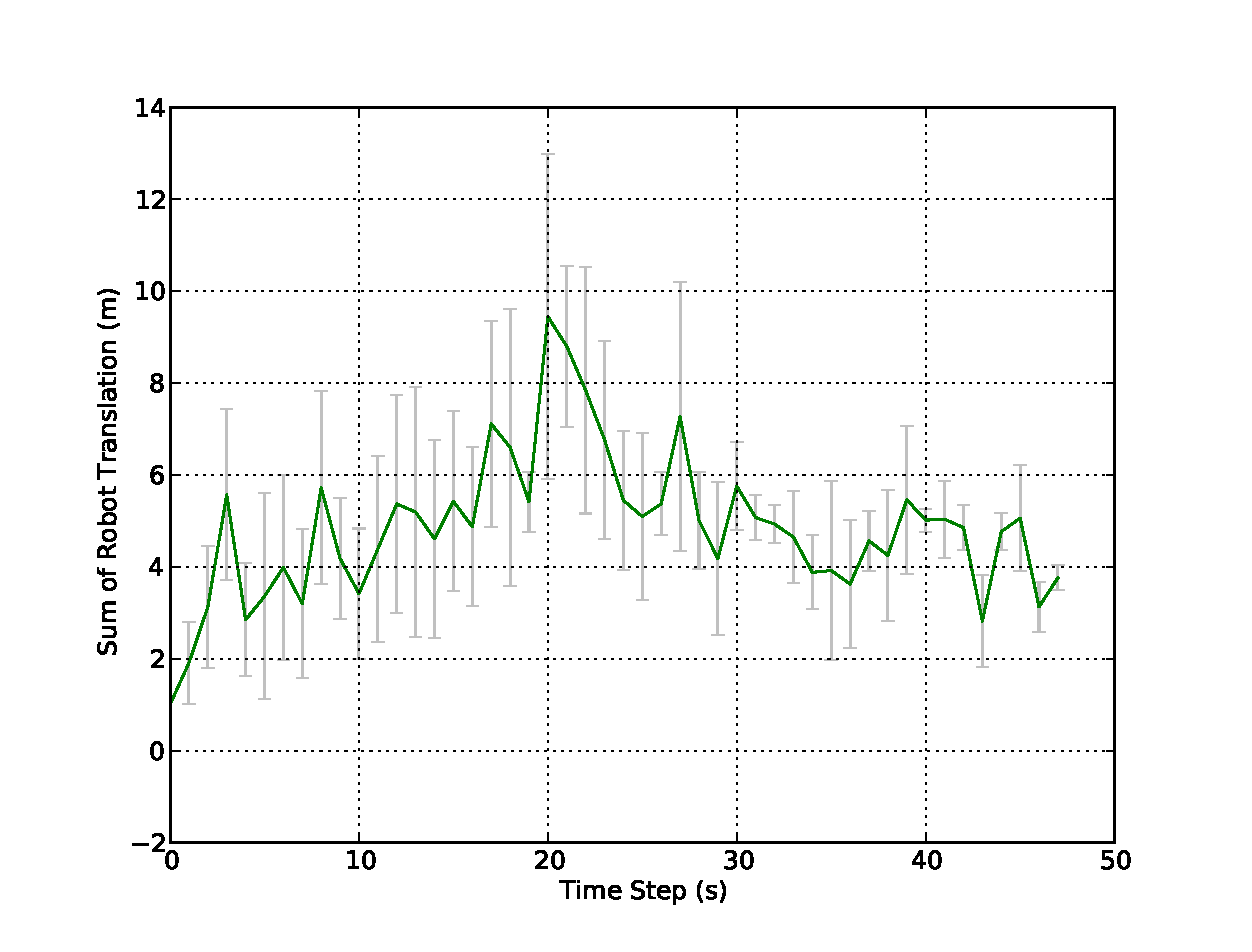
\includegraphics[height=5cm, angle=0]{images/local-1m/DeltaTranslationStat.eps}
\caption{\small Sum of translations of all robots in local mode $R_{comm}$=1m }
\label{fig:translation-stat} % Give a unique label
\end{minipage}
\end{figure*}

We have aggregated the changes in translation motion of all robots over time. Let $u_{i,q}$ and $u_{i,q+1}$ be the translations of a robot $i$ in two consecutive steps. If the difference between these two translations be $\delta u_{i}$, we can find the sum of changes of translations of all robots in $(q+1)^{th}$ step using the following equation.
\begin{equation}
\small 
\Delta U_{q+1} = \sum_{i=1}^{N} \delta u_{i, q+1} 
\label{eqn:Delta-Tr}
\end{equation}
This is plotted in Fig. \ref{fig:translation-stat}. In this plot we can see that robot translations also vary over varying task requirements of tasks. But it fails to show a consistence behaviour like previous plots.\\
%
%%% Communication load %%%
\begin{figure*}
\begin{minipage}[t]{0.5\linewidth}
\centering
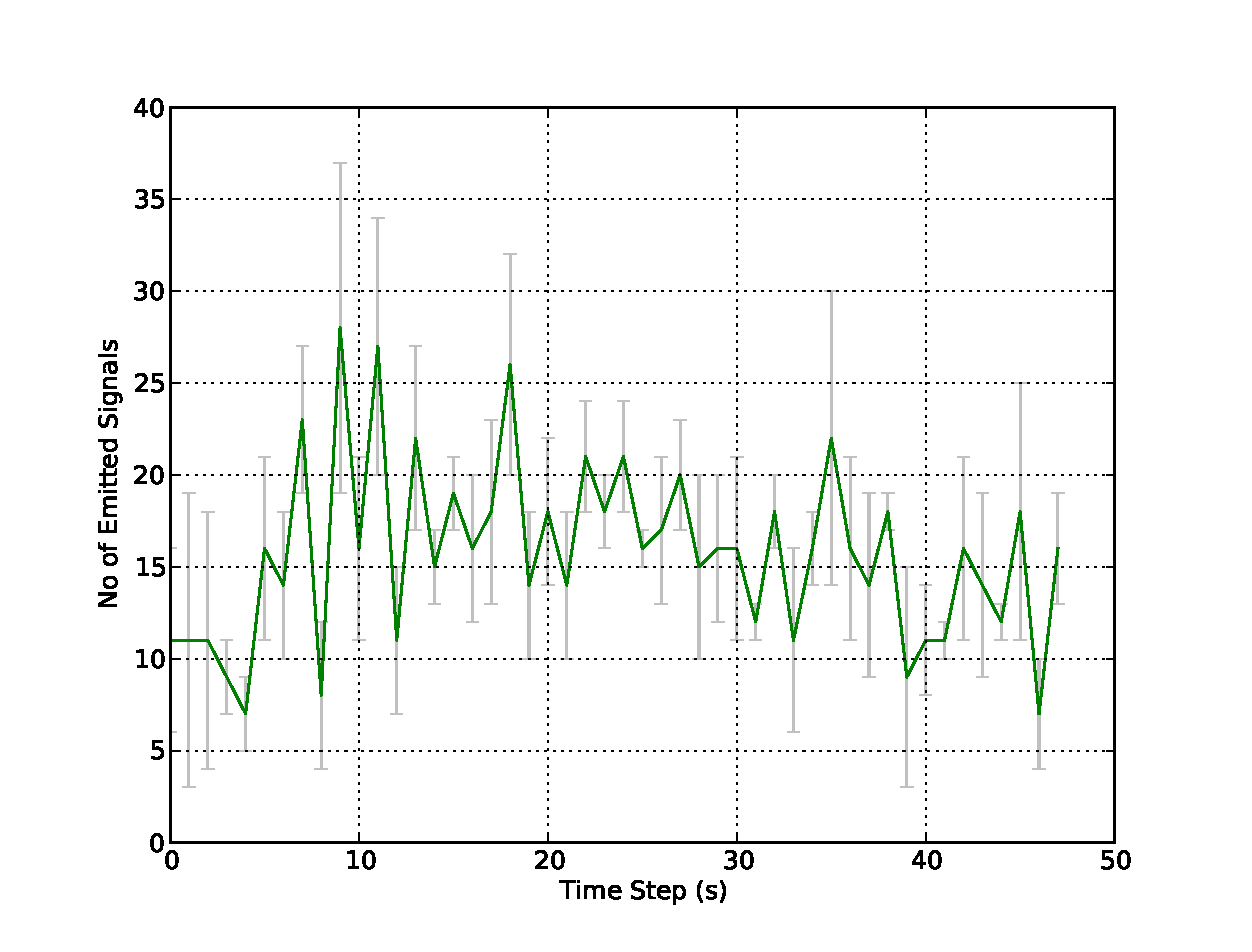
\includegraphics[height=5cm, angle=0]
{images/local-500cm/Local-500cm-SignalingFreqStat.eps}
\caption{\small Local peers' frequency of task information signalling in local mode $R_{comm}$=0.5m}
\label{fig:signal-frequency-stat} % Give a unique label
\end{minipage}
\hspace{0.5cm}
\begin{minipage}[t]{0.5\linewidth}
\centering
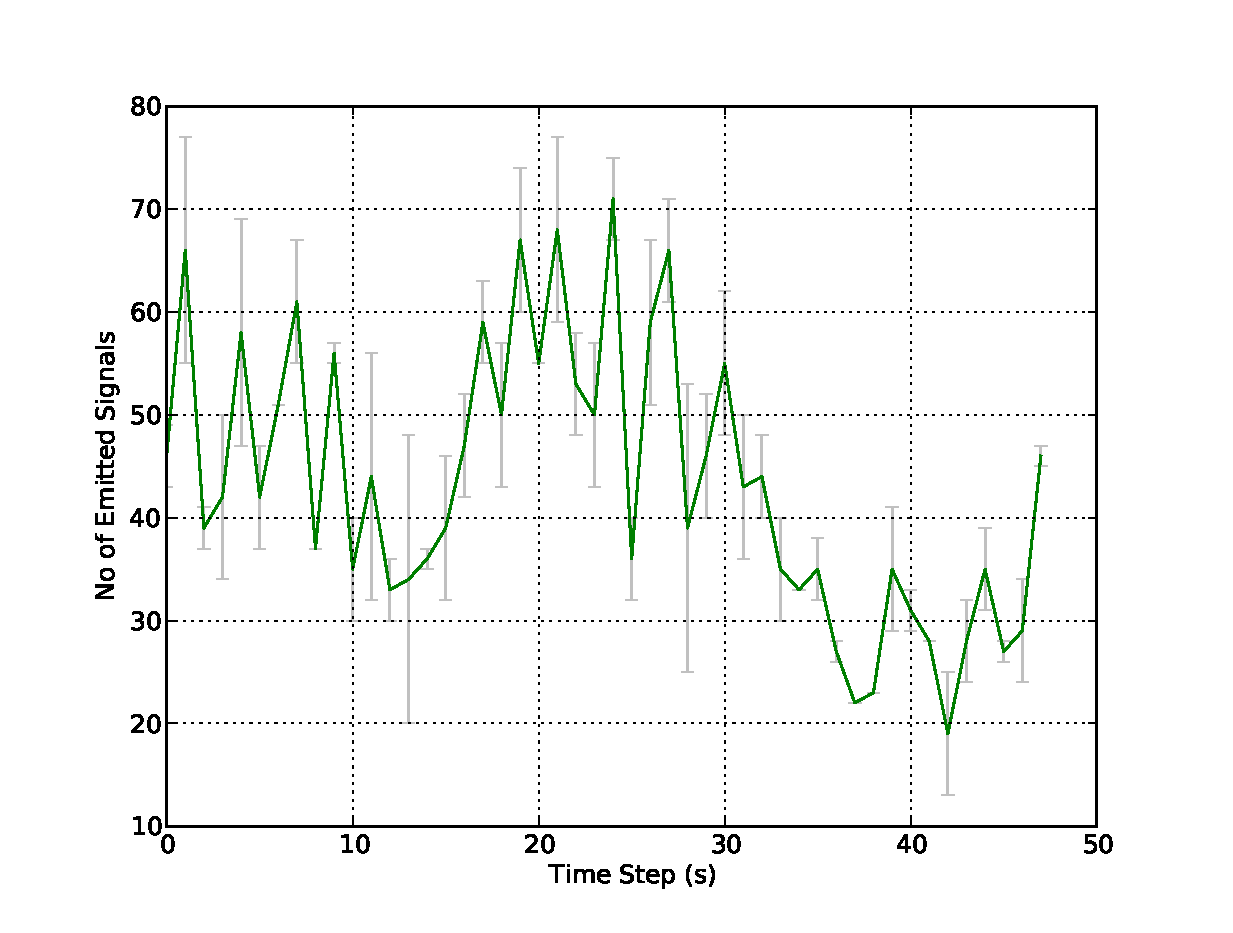
\includegraphics[height=5cm, angle=0]{images/local-1m/Local-1m-SignalingFreqStat.eps}
\caption{\small Local peers' frequency of task information signalling in local mode $R_{comm}$=1m}
\label{fig:translation-stat} % Give a unique label
\end{minipage}
\end{figure*}
%
Fig. \ref{fig:signal-frequency-stat} presents the frequency of signalling task information by TaskServer. Since the duration of each time step is 50s long and TaskServer emits signal in every 2.5s, there should be 20 signals in each step. The insignificant variation in frequency shows us the stable behaviour of D-Bus daemon over time.
%
%%%% Single- robot sensitization and translation
\begin{figure*}
\begin{minipage}[t]{0.5\linewidth}
\centering
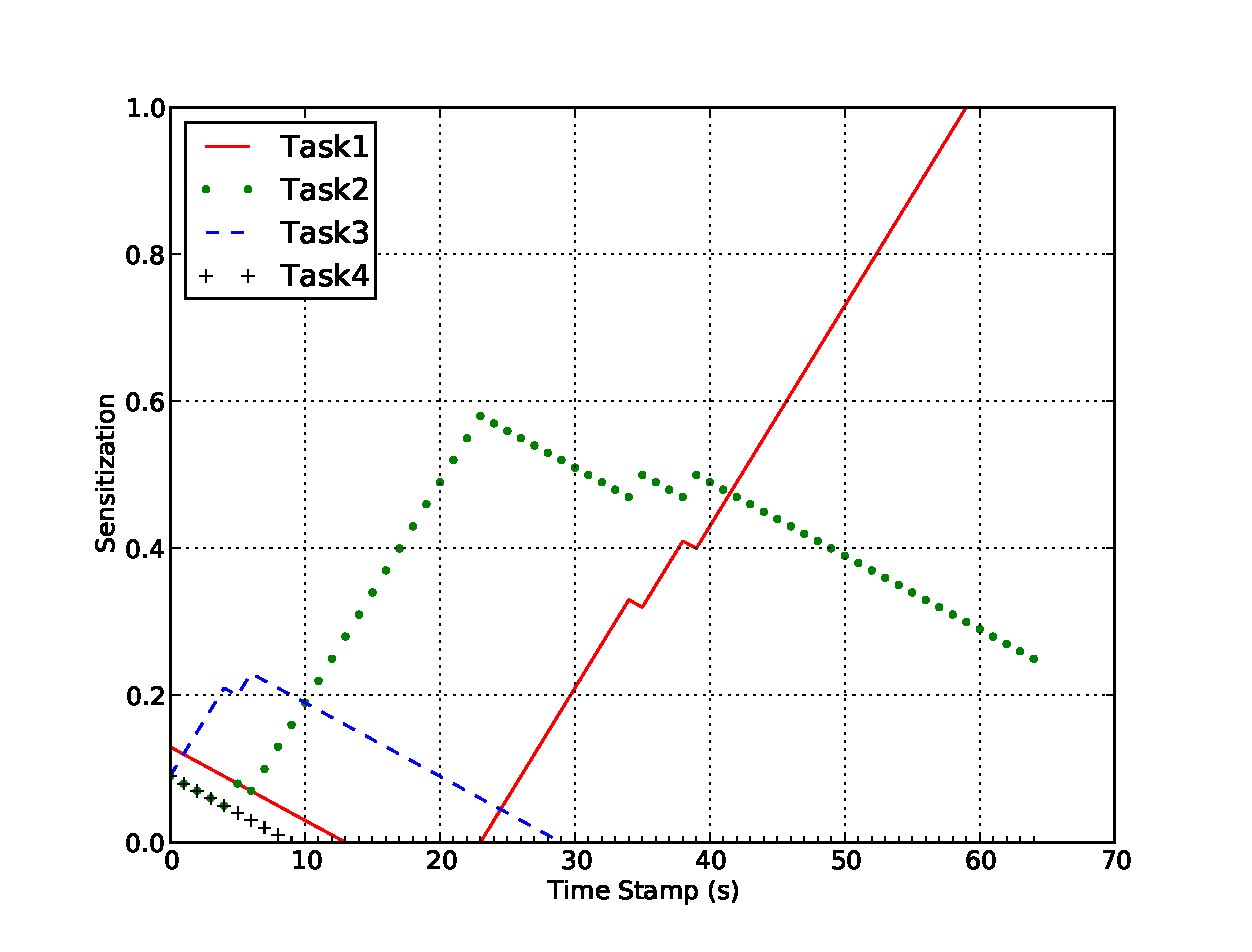
\includegraphics[height=5cm, angle=0]{images/local-500cm/PlotRobot12-Sensitizations-2010Feb16-150432.eps}
\caption{\small Task specialization of Robot12 in local mode $R_{comm}$=0.5m}
\label{fig:single-robot-sensitizations} % Give a unique label
\end{minipage} 
%%%
\begin{minipage}[t]{0.5\linewidth}
\centering
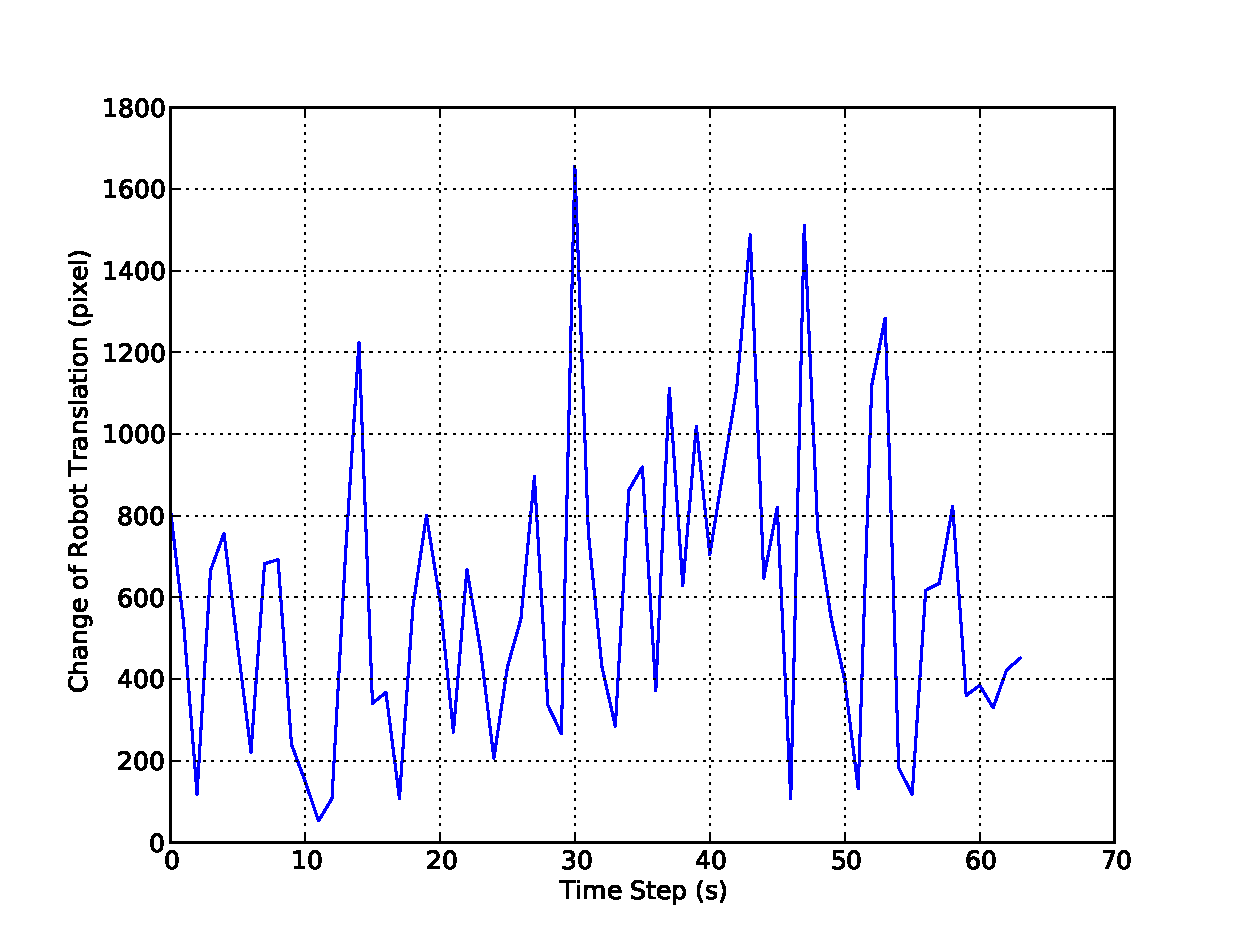
\includegraphics[height=5cm, angle=0]{images/local-500cm/DeltaRobot12-PoseAtTS-2010Feb16-150432.eps}
\caption{\small Changes in translation of Robot12 in local mode $R_{comm}$=0.5m}
\label{fig:single-robot-translation} % Give a unique label
\end{minipage}
\end{figure*}
%%%%
%%%% Single- number of peers
\begin{figure*}
\begin{minipage}[t]{0.5\linewidth}
\centering
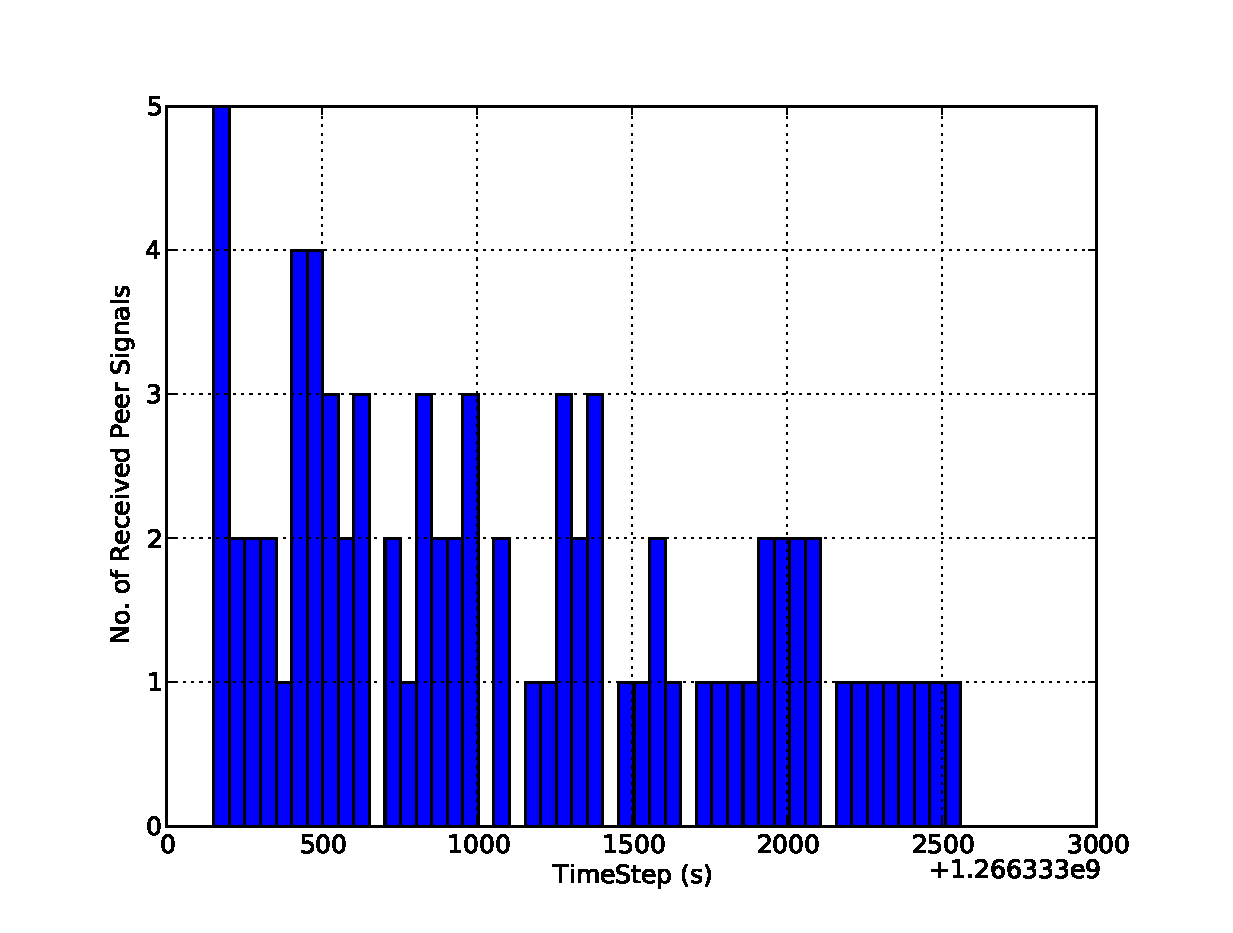
\includegraphics[height=5cm, angle=0]{images/local-500cm/Robot12-16feb-1-LocalSignals.eps}
\caption{\small Number of peer signals caught by Robot12 in local mode $R_{comm}$=0.5m}
\label{fig:single-robot-sensitizations} % Give a unique label
\end{minipage} 
%%%
\begin{minipage}[t]{0.5\linewidth}
\centering
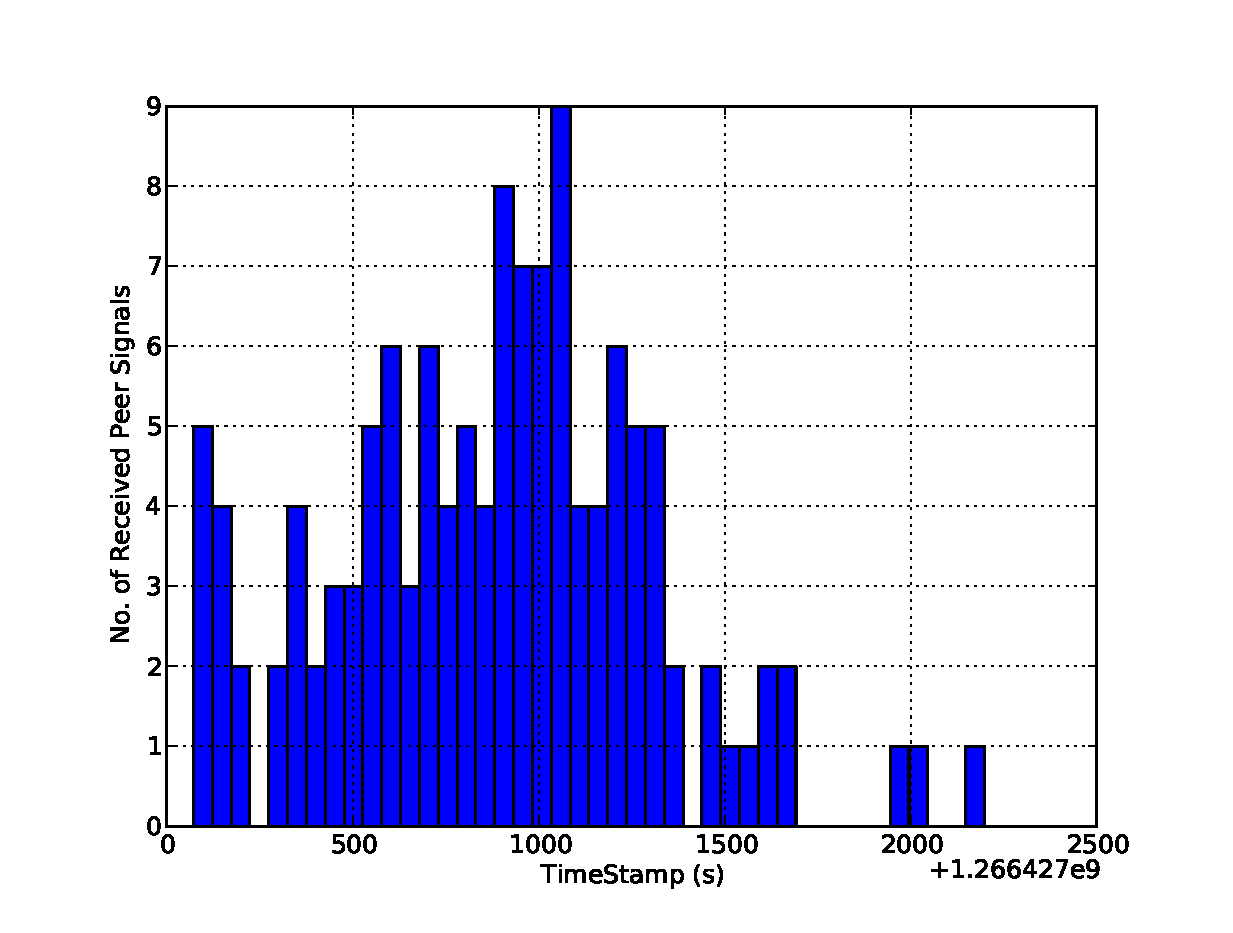
\includegraphics[height=5cm, angle=0]{images/local-1m/Robot12-17feb-3-LocalSignals.eps}
\caption{\small  Number of peer signals caught by Robot12 in local mode $R_{comm}$=1m}
\label{fig:single-robot-translation} % Give a unique label
\end{minipage}
\end{figure*}


As an example of task specialization of a robot we plotted sensitization of Robot9 in Fig. \ref{fig:single-robot-sensitizations}. It shows that this robot has specialized in Task1. The continuous learning happens from step 12 to step 42 where it has learned this task completely and forgot rest of the tasks. This behaviour is found common in all robots with varying level of sensitizations. Hence we get the linear decrease of $\Delta K$ in Fig. \ref{fig:sensitization-stat}. However, the changes in motion of this robot plotted in Fig. \ref{fig:single-robot-translation} is not stable due to the fact that robots frequently avoid dynamic obstacles and select random-walking.


%%%%%%%%%%%%%%%%%%%%%%%%%%%%%%%%%%%%%%%%%%%%%%%%%%%%%%%%%%%%%%%%%%%%%%%%%%%%%%%%
\section{CONCLUSIONS AND FUTURE WORKS}

\subsection{Conclusions}

This is a repeat.
Position figures and tables at the tops and bottoms of columns.
Avoid placing them in the middle of columns. Large figures and tables
may span across both columns. Figure captions should be below the figures;
 table captions should be above the tables. Avoid placing figures and tables
  before their first mention in the text. Use the abbreviation ``Fig. 1'',
  even at the beginning of a sentence.
Figure axis labels are often a source of confusion.
Try to use words rather then symbols. As an example write the quantity ``Inductance",
 or ``Inductance L'', not just.
 Put units in parentheses. Do not label axes only with units.
 In the example, write ``Inductance (mH)'', or ``Inductance L (mH)'', not just ``mH''.
 Do not label axes with the ratio of quantities and units.
 For example, write ``Temperature (K)'', not ``Temperature/K''.


\subsection{Future Works}

This is a repeat.
Position figures and tables at the tops and bottoms of columns.
Avoid placing them in the middle of columns. Large figures and tables
may span across both columns. Figure captions should be below the figures;
 table captions should be above the tables. Avoid placing figures and tables
  before their first mention in the text. Use the abbreviation ``Fig. 1'',
  even at the beginning of a sentence.
Figure axis labels are often a source of confusion.
Try to use words rather then symbols. As an example write the quantity ``Inductance",
 or ``Inductance L'', not just.
 Put units in parentheses. Do not label axes only with units.
 In the example, write ``Inductance (mH)'', or ``Inductance L (mH)'', not just ``mH''.
 Do not label axes with the ratio of quantities and units.
 For example, write ``Temperature (K)'', not ``Temperature/K''.

%%%%%%%%%%%%%%%%%%%%%%%%%%%%%%%%%%%%%%%%%%%%%%%%%%%%%%%%%%%%%%%%%%%%%%%%%%%%%%%%
\section{ACKNOWLEDGMENTS}

The authors gratefully acknowledge the contribution of National Research Organization and reviewers' comments.


%%%%%%%%%%%%%%%%%%%%%%%%%%%%%%%%%%%%%%%%%%%%%%%%%%%%%%%%%%%%%%%%%%%%%%%%%%%%%%%%

References are important to the reader; therefore, each citation must be complete and correct. If at all possible, references should be commonly available publications.

\begin{thebibliography}{99}

\bibitem{c1}
J.G.F. Francis, The QR Transformation I, {\it Comput. J.}, vol. 4, 1961, pp 265-271.

\bibitem{c2}
H. Kwakernaak and R. Sivan, {\it Modern Signals and Systems}, Prentice Hall, Englewood Cliffs, NJ; 1991.

\bibitem{c3}
D. Boley and R. Maier, "A Parallel QR Algorithm for the Non-Symmetric Eigenvalue Algorithm", {\it in Third SIAM Conference on Applied Linear Algebra}, Madison, WI, 1988, pp. A20.

\end{thebibliography}

\end{document}
